Στην παρούσα ενότητα παρουσιάζουμε τρεις διαφορετικές μεθόδους επιχείρησης
ελάττωσης του σφάλματος εκτίμησης κατάστασης μίας κινητής βάσης ρομπότ, η οποία
φέρει ως εξωδεκτικό αισθητήρα έναν αισθητήρα αποστάσεων τύπου lidar, ο οποίος
συλλαμβάνει δισδιάστατες μετρήσεις.  Η εκτίμηση της στάσης της γίνεται μέσω
του φίλτρου σωματιδίων, και οι παραπάνω μέθοδοι στοχεύουν στην επίλυση του
προβλήματος \ref{prob:02_02:the_problem} μέσω (α) διαλογής σωματιδίων του
πληθυσμού του φίλτρου (ενότητα \ref{subsection:02_02_03:01}), (β) ευθυγράμμισης
πραγματικών με εικονικές σαρώσεις (ενότητα \ref{subsection:02_02_03:02}),
και (γ) ανάδρασης του αποτελέσματος της ευθυγράμμισης στον πληθυσμό του φίλτρου
(ενότητα \ref{subsection:02_02_03:03}).

%%%%%%%%%%%%%%%%%%%%%%%%%%%%%%%%%%%%%%%%%%%%%%%%%%%%%%%%%%%%%%%%%%%%%%%%%%%%%%%%
\subsection{Μέσω διαλογής σωματιδίων}
\label{subsection:02_02_03:01}

Έστω ένα ρομπότ κινητής βάσης του πεδίου εφαρμογής \ref{scope}. Τα φίλτρα
σωματιδίων διατηρούν την εκτίμηση της στάσης του σε κάθε χρονικό βήμα $t$,
$\hat{\bm{x}}_t (x, y, \theta)$, εντός ενός χάρτη $\bm{M}$, με τη μορφή ενός
συνόλου από ``σωματίδια", δηλαδή τυχαία δείγματα από την κατανομή πιθανότητας
$p(\bm{x}_t | \bm{z}_t, \bm{M})$. Εδώ $\bm{z}_t$ είναι το διάνυσμα
παρατηρήσεων, οι οποίες ανιχνεύονται τη χρονική στιγμή $t$ από το ρομπότ μέσω
της χρήσης των αισθητήρων του, και οι οποίοι, στα συμφραζόμενα της παρούσας
διατριβής, αποτελούνται αποκλειστικά από έναν αισθητήρα αποστάσεων τύπου lidar,
ο οποίος συλλαμβάνει δισδιάστατες μετρήσεις. H αναπαράσταση της κατανομής
$p(\bm{x}_t | \bm{z}_t, M)$ από ένα σύνολο δειγμάτων οφείλεται στην ουσιαστική
δυϊκότητα μεταξύ των δύο \cite{Smith1992}.

Αυτή η ιδιότητα των φίλτρων σωματιδίων τούς επιτρέπει την ικανότητα
αναπαράστασης πολυτροπικών (multi-modal) κατανομών---μια προϋπόθεση για τον
εντοπισμό της στάσης του ρομπότ βάσει καθολικής αβεβαιότητος---αλλά, με την
ίδια λογική, καθιστά ασαφή την απάντηση στο ερώτημα του συνδυασμού όλων των
πιθανών υποθέσεων (κάθε σωματίδιο εκφράζει μια διακριτή υπόθεση για την
κατάσταση του ρομπότ εντός του $\bm{M}$) μέσω του υπολογισμού μιας ενιαίας
εκτίμησης της στάσης του ρομπότ. Στα φίλτρα Kalman, σε αντίθεση, τα οποία είναι
αυστηρά μονοτροπικoί (uni-modal) εκτιμητές, για την εκτίμηση του φίλτρου αρκεί
το διάνυσμα της στάσης και η συνδιακύμανση της για τον υπολογισμό της εκτίμησης
της κατάστασης $\bm{x}_t$ \cite{Maybeck1979}. Αντιθέτως, στα φίλτρα σωματιδίων
δεν υπάρχει \textit{μία} ενιαία λύση κλειστής μορφής για αυτό το πρόβλημα. Η
επικρατούσα προσέγγιση για τον υπολογισμό της εκτιμώμενης στάσης είναι έμμεση,
και υποθέτει την ταυτοποίηση μέσα στην κατανομή των σωματιδίων εκείνης της
υποκατανομής με το μεγαλύτερο συνολικό βάρος (ενότητα \ref{subsec:01_01_02_3}),
προτού στη συνέχεια προχωρήσει στον υπολογισμό του σταθμισμένου κέντρου της.
Στην περίπτωση όπου η εκτίμηση έχει συγκλίνει και η κατανομή έχει γίνει
μονοτροπική, αυτή η προσέγγιση είναι ισοδύναμη με τη εξαγωγή της μέσης τιμής
των εκτιμήσεων όλων των σωματιδίων, σταθμισμένη με το ατομικό βάρος του
καθενός.

Η βιβλιογραφία σχετικά με την εξαγωγή της τελικής εκτίμησης στάσης ενός φίλτρου
σωματιδίων με βάση κάποια συγκεκριμένα χαρακτηριστικά τους είναι μάλλον ισχνή:
μόνο τα \cite{Liemhetcharat2010} και \cite{Coltin2013} επικεντρώνονται σε αυτό
το έργο, και στα συμφραζόμενα των ανθρωποειδών ρομπότ, λόγω της ανάγκης
ελάττωσης του αρκούντως υψηλού σφάλματος εκτίμησης της στάσης τους, η οποία
προκύπτει από τη χρήση μικρών σε μέγεθος και θορυβωδών αισθητήρων.  Αρχικά, τη
χρονική στιγμή $t$ προσδιορίζουν το σωματίδιο με το μεγαλύτερο βάρος μέσα σε
συγκεκριμένα όρια μεταφορικής και περιστροφικής απόστασης από την εκτίμηση της
στάσης τη χρονική στιγμή $t-1$. Οι συγγραφείς εκτελούν την επιλογή με αυτόν τον
τρόπο προκειμένου να αμβλυνθεί η ασυνέχεια της εκτίμησης της στάσης στο χώρο.
Στη συνέχεια η τελική στάση υπολογίζεται ως το κεντροειδές όλων των σωματιδίων
εντός μιας προκαθορισμένης ακτίνας γύρω από αυτό το σωματίδιο, εάν το βάρος της
συστάδας τους ξεπερνά ένα κατώφλι βάρους. Ωστόσο, εάν η τιμή του είναι
μικρότερη από το κατώφλι, η τελική εκτίμηση του φίλτρου εξάγεται ως το
σωματίδιο με το μεγαλύτερο βάρος. Στη συνέχεια θα δείξουμε ότι αυτή η δεύτερη
απόφαση, ενώ διαισθητικά ορθή, στην πραγματικότητα δεν είναι σοφή και,
επομένως, δεν αποτελεί βιώσιμη λύση για επέκταση σε άλλες συνθήκες πέρα από τα
πλαίσια αυτών των δύο έργων.

Στα φίλτρα σωματιδίων κάθε σωματίδιο χαρακτηρίζεται από έναν δείκτη
ακρίβειας-βαρύτητας, ο οποίος ονομάζεται ``βάρος" του κάθε σωματιδίου. Το βάρος
$w_t^i$ ενός σωματιδίου $i$ τη χρονική στιγμή $t$ ποσοτικοποιεί την πιθανότητα
το ρομπότ να έχει παρατηρήσει τις πραγματικές μετρήσεις $\bm{z}_t$ από την
εκτιμώμενη στάση του σωματιδίου $\hat{\bm{x}}_t^i(x_i, y_i, \theta_i)$.  Αυτό
σημαίνει ότι, δεδομένου ενός χάρτη $\bm{M}$ πιστότητας στη λειτουργική
κατάσταση του περιβάλλοντος, όσο πιο ακριβής είναι η εκτίμηση της στάσης του
ρομπότ $\hat{\bm{x}}_t^i(x_i, y_i, \theta_i)$, τόσο πιο κοντά είναι στην
πραγματική του στάση $\bm{x}_t(x,y,\theta)$, και επομένως τόσο μεγαλύτερη είναι
η συμφωνία των πραγματικών μετρήσεων $\bm{z}_t$ και των προβλεπόμενων μετρήσεων
$\hat{\bm{z}}_t^i$. Επομένως, θεωρητικά, υπάρχει μια άμεση δυσαναλογία μεταξύ
του σφάλματος εκτίμησης ενός σωματιδίου (η απόκλιση της εκτιμώμενης στάσης από
την πραγματική της τιμή) και της τιμής του βάρους του: όσο μικρότερο είναι το
σφάλμα εκτίμησης της στάσης του, τόσο μεγαλύτερο είναι το βάρος του, και
αντίστροφα.

Αυτό το τελικό συμπέρασμα, σε αντιδιαστολή με την κυρίαρχη προσέγγιση εξαγωγής
της εκτίμησης του φίλτρου, αποτέλεσε το κίνητρό μας για τη διερεύνηση της
εξαγωγής της εκτίμησης της στάσης του μέσω άλλων μεθόδων από την επικρατούσα.
Θεωρητικά, λοιπόν, θα περιμέναμε ότι η επιλογή σωματιδίων με υψηλό βάρος (που
ισοδυναμεί με την απόρριψη σωματιδίων με χαμηλό βάρος---σωματίδια των οποίων η
εκτίμηση της στάσης εξηγεί τις μετρήσεις $\bm{z}_t$ με λιγότερο ικανοποιητικό
τρόπο σε σύγκριση με άλλα σωματίδια του πληθυσμού) για τον υπολογισμό της
σύνθετης εκτίμησης του φίλτρου θα είχε ως αποτέλεσμα καλύτερες εκτιμήσεις
στάσης, δηλαδή εκτιμήσεις με μικρότερο σφάλμα ως προς τη στάση ρομπότ σε κάθε
χρονικό βήμα. Δεδομένου ότι το βάρος ενός σωματιδίου είναι ένα καθορισμένο,
ποσοτικοποιήσιμο, και οριστικό μέτρο της ευθυγράμμισης των μετρήσεων των
αισθητήρων και των αναμενόμενων μετρήσεων τους, και δεδομένου ότι η τιμή που
αποδίδεται στο βάρος ενός σωματιδίου γίνεται με αναλογικό τρόπο, όλες οι
μέθοδοι επιλογής σωματιδίων για την εξαγωγή της εκτίμησης του φίλτρου που θα
καλύψουμε είναι βασισμένες στο βάρος. Περιορίζουμε τις μεθόδους επιλογής μας σε
προσεγγίσεις με βάση το βάρος διότι στα πλαίσια των φίλτρων σωματιδίων το βάρος
ενός σωματιδίου είναι ο μοναδικός δείκτης της ακρίβειας (και συνεπώς του
σφάλματος) της εκτίμησής του.

Έστω $\bm{P}_t$ το σύνολο του πληθυσμού των σωματιδίων τη χρονική στιγμή $t$.
Τότε $\bm{P}_t \equiv \{(\hat{\bm{x}}_t^i, w_t^i)\}, i =
0,1,\dots,|\bm{P}_t|-1$, όπου $\hat{\bm{x}}_t^i$ είναι η εκτίμηση του $i$-οστού
σωματιδίου της στάσης του ρομπότ τη χρονική στιγμή $t$, και $w_t^i$ είναι το
βάρος που σχετίζεται με το σωματίδιο $i$ την ίδια χρονική στιγμή.  Επιπλέον,
έστω $\overline{W}_t = \dfrac{1}{|\bm{P}_t|}\sum\limits_{i=0}^{|\bm{P}_t|-1}
w_t^i$ το μέσο βάρος των σωματιδίων του $\bm{P}_t$. Στη συνέχεια διακρίνουμε
δύο διακριτές μεθόδους επιλογής: (α) απόλυτες και (β) σχετικές μεθόδους.
Στις μεθόδους απόλυτης επιλογής ένα απόλυτο ποσοστό του πληθυσμού
$\bm{P}_t$ καλείται να ψηφίσει για την εκτίμηση της στάσης του ρομπότ τη
χρονική στιγμή $t$. Η επικρατούσα μέθοδος υπολογισμού της στάσης είναι μια
ειδική περίπτωση της απόλυτης επιλογής, όπου το ποσοστό των επιλεγμένων
σωματιδίων είναι $100\%$.  Στις μεθόδους σχετικής επιλογής τα σωματίδια
επιλέγονται για ψηφοφορία υπό την προϋπόθεση ικανοποίησης κάποιας σχέσης των
βαρών τους $w_t^i$ με το συνολικό βάρος του πληθυσμού $\overline{W}_t$: για
παράδειγμα, μόνο τα σωματίδια των οποίων $w_t^i > \overline{W}_t$ επιλέγονται
να έχουν λόγο στην συνολική εκτίμηση της στάσης του φίλτρου. Ο Αλγόριθμος
\ref{alg:particle_selection} απεικονίζει σε ψευδοκώδικα τη διαδικασία επιλογής
σωματιδίων για την εξαγωγή της τελικής εκτίμησης του φίλτρου, η οποία στοχεύει
στην επίλυση του προβλήματος \ref{prob:02_02:the_problem} υπό την Παραδοχή
\ref{assumption:02_02_01:01}.

\begin{algorithm}[h]
  \caption{\texttt{particle\_selection}}
  \label{alg:particle_selection}
  \begin{spacing}{1.2}
  \begin{algorithmic}[1]
    \REQUIRE $\bm{P}_t \equiv \{(\hat{\bm{x}}_t^i, w_t^i)\}$, selection\_manner, fraction
    \ENSURE pose estimate $\hat{\bm{x}}_t$
    \STATE \texttt{assert} selection\_manner = \texttt{absolute} $|\ |$ \texttt{relative}
    \STATE \texttt{assert} fraction $\in [0,1]$
    \IF {selection\_manner = \texttt{absolute}}
      \STATE $\bm{P}_t^\prime \leftarrow $ \texttt{sort} $\bm{P}_t$ by weight $w_t^i$, descending
      \IF {fraction $> 0.0$}
        \STATE $\bm{P}_t^{\prime\prime} \leftarrow \bm{P}_t^\prime[0: \lfloor\text{fraction}\cdot|\bm{P}_t^\prime| \rfloor - 1]$
      \ELSE
        \STATE $\bm{P}_t^{\prime\prime} \leftarrow \bm{P}_t^\prime[0]$
      \ENDIF
    \ENDIF
    \IF {selection\_manner = \texttt{relative}}
      \STATE $\overline{W}_t \leftarrow \dfrac{1}{|\bm{P}_t|}\sum\limits_{i=0}^{|\bm{P}_t|-1} w_t^i$
      \STATE $\bm{P}_t^{\prime\prime} \leftarrow \hat{\bm{x}}_t^i : w_t^i > \overline{W}_t$
    \ENDIF
    \STATE $\hat{\bm{x}}_t \leftarrow (0,0,0)$
    \FOR {$j = 0 : |\bm{P}_t^{\prime\prime}|-1$}
      \STATE $\hat{\bm{x}_t} \leftarrow \hat{\bm{x}_t} + \bm{P}_t^{\prime\prime}[j].w_t \cdot \bm{P}_t^{\prime\prime}[j].\hat{\bm{x}}_t$
    \ENDFOR
    \RETURN $\hat{\bm{x}}_t$
  \end{algorithmic}
  \end{spacing}
\end{algorithm}

Στον Αλγόριθμο \ref{alg:particle_selection}, αν επιλεγεί ο απόλυτος τρόπος
επιλογής (absolute), ο πληθυσμός σωματιδίων ταξινομείται πρώτα με βάση το βάρος
του καθενός σε φθίνουσα σειρά (γραμμή 4), και στο ταξινομημένο σύνολο
σωματιδίων δίνεται η ονομασία $\bm{P}_t^\prime$. Στη συνέχεια τα πρώτα $\lfloor
\text{fraction}\cdot|\bm{P}_t^\prime| \rfloor$ σωματίδια λαμβάνονται υπόψιν
προς υπολογισμό της τελικής εκτίμησης, όπου το fraction $\in [0,1]$ εκφράζει
την αναλογία των σωματιδίων που θα ληφθούν υπόψη (γραμμή 6)---η σύμβαση
fraction $=0$ προορίζεται για την επιλογή του σωματιδίου με το μεγαλύτερο βάρος
μεταξύ όλων του συνόλου $\bm{P}_t$. Ο συμβολισμός $\bm{P}_t^\prime[a]$ δηλώνει
το σωματίδιο του $\bm{P}_t^\prime$ με δείκτη $a$, και ο συμβολισμός
$\bm{P}_t^\prime[a$:$b]$ δηλώνει το σύνολο των σωματιδίων που αποτελούνται από
τα στοιχεία του $\bm{P}_t^\prime$ από τον δείκτη $a$ μέχρι και τον δείκτη $b$.
Από την άλλη πλευρά, αν επιλεγεί η σχετική επιλογή (relative), πρώτα
υπολογίζεται το μέσο βάρος του πληθυσμού (γραμμή 12), και στη συνέχεια όλα τα
σωματίδια των οποίων το βάρος υπερβαίνει αυτή την τιμή περιλαμβάνονται στο
σύνολο σωματιδίων που μεταφέρεται εμπρός (γραμμή 13).  Και στις δύο περιπτώσεις
το σύνολο $\bm{P}_t^{\prime\prime}$ περιλαμβάνει τις υποθέσεις του συνόλου
σωματιδίων που έχουν επιλεγεί για να προσδώσουν την τελική εκτίμηση του
φίλτρου.  Στη συνέχεια υπολογίζεται ο σταθμισμένος κατά βάρος μέσος όρος των
εκτιμήσεων στάσης αυτού του συνόλου (γραμμή 17) και η προκύπτουσα στάση
θεωρείται ως η έξοδος του συστήματος επιλογής σωματιδίων. Ο συμβολισμός
$\bm{P}_t^{\prime\prime}[j].a$ για το σύνολο σωματιδίων
$\bm{P}_t^{\prime\prime}$ δηλώνει τη συνιστώσα $a$ (δηλαδή το βάρος $w_t$ ή την
εκτίμηση της στάσης $\hat{\bm{x}}_t$) του στοιχείου του
$\bm{P}_t^{\prime\prime}$ στο δείκτη $j$ για τη χρονική στιγμή $t$.

Ένα εύλογο ερώτημα που μπορεί να τεθεί είναι γιατί δεν κρατάμε το συνολικό
μέγεθος του πληθυσμού στο κλάσμα επιλογής fraction $\cdot |\bm{P}_t|$ ώστε να
απαλλαγούμε συνολικά από τον μηχανισμό επιλογής. Αυτό θα ήταν δυνητικά
καταστροφικό, καθώς η διατήρηση ενός χαμηλότερου αριθμό σωματιδίων θα αύξανε
τον κίνδυνο αποστέρησης σωματιδίων (particle deprivation)
\cite{thrun2005probabilistic}. Έπειτα, καθώς το μέγεθος του πληθυσμού αυξάνει,
αυξάνεται και η πιστότητα της εκ των υστέρων πιθανότητας εκτίμησης της στάσης
του ρομπότ (εξ. (\ref{eq:pf_posterior})) ως προς την αληθινή του στάση.
Αντίστροφα, όσο μικρότερος είναι ο αριθμός των σωματιδίων του φίλτρου τόσο
μεγαλύτερη είναι η πιθανότητα απόκλισης της εκτίμησής του. Με τον παραπάνω
τρόπο προσέγγισης προφυλασσόμαστε και από τη στέρηση σωματιδίων (διατηρώντας
ένα αυξημένο μέγεθος του πληθυσμού) και ταυτόχρονα χρησιμοποιούμε ένα καθεστώς
επιλογής ώστε το σύστημα να αυξάνει την ακρίβειά του χωρίς να θυσιάζει την
ποιότητα/ακρίβεια της εκ των υστέρων πιθανότητας εκτίμησης της στάσης του
ρομπότ ή την ευστάθεια του φίλτρου.

Αν και θεωρητικά οι παραπάνω μέθοδοι επιλογής είναι ορθές (δεδομένου ότι η
επιλογή βαρύτερων σωματιδίων, η οποία απορρίπτει τα σωματίδια με περισσότερο
ανακριβή εκτίμηση, βελτιώνει την ποιότητα της συνολικής εκτίμησης), στην πράξη
(ενότητα \ref{subsection:02_02_04:03}) παρατηρούμε ποικίλα ή δυσμενή
αποτελέσματα, τα οποία μπορούν να αποδοθούν (α) στην απώλεια συνολικής
πληροφορίας, (β) στον υψηλότερο βαθμό επιρροής που αποκτούν τα σωματίδια όταν η
πληθικότητα του συνόλου ψηφοφορίας μειώνεται, ή/και (γ) στην απομάκρυνση
σωματιδίων με σχεδόν συμμετρικές θέσεις που υπάρχουν στον πληθυσμό λόγω της
τυχαιότητας που εισάγεται κατά τη διάρκεια του φίλτρου κατά τη φάση πρόβλεψης
(prediction stage) του φίλτρου.

Στην επόμενη ενότητα αιτιολογούμε πώς το χάσμα μεταξύ της εκτιμώμενης στάσης
του φίλτρου και της πραγματικής στάσης μπορεί να μειωθεί με τον επιπρόσθετο
τρόπο της ευθυγράμμισης εικονικών μετρήσεων που λαμβάνονται εντός του χάρτη
$\bm{M}$ από την πρώτη με πραγματικές μετρήσεις που λαμβάνονται από τον φυσικό
αισθητήρα από την δεύτερη.

%%%%%%%%%%%%%%%%%%%%%%%%%%%%%%%%%%%%%%%%%%%%%%%%%%%%%%%%%%%%%%%%%%%%%%%%%%%%%%%%
\subsection{Μέσω ευθυγράμμισης πραγματικών μετρήσεων με σαρώσεις χάρτη}
\label{subsection:02_02_03:02}

Στην παρούσα μελέτη επιδιώκουμε να βελτιώσουμε την εκτίμηση ενός φίλτρου
σωματιδίων με διάφορα μέσα: στην προηγούμενη ενότητα αναλύσαμε θεωρητικά τον
τρόπο με τον οποίο η επιλογή σωματιδίων με μεγάλη βαρύτητα για τον προσδιορισμό
της στάσης εξόδου του φίλτρου στρέφει το φίλτρο στον υπολογισμό ακριβέστερων
εκτιμήσεων. Στην παρούσα ενότητα θα εξετάσουμε πώς η ευθυγράμμιση πραγματικών
με εικονικές μετρήσεις-σαρώσεις μπορεί να χρησιμοποιηθεί προσθετικά στο φίλτρο
σωματιδίων (ή σε οποιαδήποτε άλλη τεχνική εντοπισμού μέσω της χρήσης
αισθητήρα lidar), έτσι ώστε η τελική εκτίμηση του συστήματος να
πλησιάζει περισσότερο στην αληθινή στάση του ρομπότ, και συνεπώς να επιλύει
το πρόβλημα \ref{prob:02_02:the_problem}. Αυτή η τεχνική είναι εμπνευσμένη από
το \cite{Vasiljevic2016a} και καλύπτεται λεπτομερέστερα εδώ για τους λόγους
σχολαστικότητας και πληρότητας.

Έστω ότι ένα ρομπότ του πεδίου εφαρμογής \ref{scope} φέρει έναν αισθητήρα
αποστάσεων τύπου lidar δισδιάστατων μετρήσεων, και ότι λειτουργεί σε ένα
καθορισμένο περιβάλλον το οποίο αναπαρίσταται μέσω ενός δισδιάστατου χάρτη
$\bm{M}$. Έστω επίσης ότι τη χρονική στιγμή $t$ το φίλτρο σωματιδίων έχει
εξάγει μια εκτιμώμενη στάση $\hat{\bm{x}}_t(x,y,\theta)$ χρησιμοποιώντας κάποια
μέθοδο επιλογής σωματιδίων, και ότι μία μέτρηση $\mathcal{S}^R_t$ μέσω του
αισθητήρα, η οποία έχει ληφθεί από την πραγματική στάση του ρομπότ, είναι
επίσης διαθέσιμη τη χρονική στιγμή $t$. Τότε, αν συλλάβουμε μια εικονική σάρωση
$\mathcal{S}^V_t$ από την εκτιμώμενη στάση $\hat{\bm{x}}_t$ (Ορισμός
\ref{def:map_scan}), η οποία είναι το αποτέλεσμα της προσομοίωσης της αρχής
λειτουργίας του πραγματικού αισθητήρα \textit{αλλά αυτή τη φορά στο χάρτη
$\bm{M}$} για το ίδιο γωνιακό εύρος και μέγιστη αισθητή απόσταση του, είναι
δυνατόν με την ευθυγράμμιση των δύο σαρώσεων (Ορισμός \ref{def:smsm})
να προκύψει ο μετασχηματισμός $\bm{q}_t$ ο οποίος, αν εφαρμοστεί στην εκτίμηση
$\hat{\bm{x}}_t$, θα την κάνει συμπίπτει με την πραγματική στάση $\bm{x}_t$.

Ωστόσο, λόγω (α) της παρουσίας θορύβου στις μετρήσεις $\mathcal{S}^R_t$ του
αισθητήρα, (β) της ενδεχόμενης αναντιστοιχίας μεταξύ του χάρτη $\bm{M}$ του
περιβάλλοντος λειτουργίας και του ίδιου του περιβάλλοντος, η οποία οδηγεί στην
πρακτική παρουσία θορύβου στις μετρήσεις της σάρωσης $\mathcal{S}^V_t$, (γ) της
ενδεχόμενης διακριτής φύσης του χάρτη (εάν ο $\bm{M}$ είναι ένας χάρτης
πλέγματος πεπερασμένης ανάλυσης), και (δ) του γεγονότος ότι ο χρησιμοποιούμενος
αλγόριθμος ευθυγράμμισης δεν είναι απαραίτητα ένας τέλειος τελεστής, αναμένουμε
ότι αυτό που πραγματικά θα συμβαίνει είναι ότι η εφαρμογή του $\bm{q}_t$ στην
εκτίμηση της στάσης $\hat{\bm{x}}_t$ θα μετακινήσει την εκτίμηση αυτή σε μία
γειτονιά της πραγματικής στάσης και όχι ακριβώς σε αυτήν. Το προκύπτον σφάλμα
εκτίμησης εξαρτάται από ένα πλήθος παραμέτρων, μεταξύ άλλων, από την ποιότητα
της οδομετρίας του ρομπότ, την αντιστοιχία του κινηματικού μοντέλου του ρομπότ
με την πραγματική δυναμική του, το μέγεθος του θορύβου του αισθητήρα, την
ανάλυση του χάρτη, την ακρίβεια του αλγορίθμου ευθυγράμμισης στην εκτίμηση του
μετασχηματισμού μεταξύ των δύο συνόλων σημείων, το μέγεθος του πληθυσμού των
σωματιδίων, την κατάσταση του χάρτη σε συνδυασμό με την ικανότητα του
αλγορίθμου ευθυγράμμισης στο να απορρίπτει ακραίες ή μη-αντιστοιχούσες τιμές,
το μέγιστο εύρος του αισθητήρα σάρωσης, καθώς και το γωνιακό του εύρος.

Στην επόμενη ενότητα αιτιολογούμε πώς το σφάλμα της εκτιμώμενης στάσης
του MCL σε συνδυασμό με έναν αλγόριθμο ευθυγράμμισης πραγματικών και εικονικών
σαρώσεων μπορεί να μειωθεί περαιτέρω με την ανάδραση της εκτίμησης του
συνολικού τους συστήματος πίσω στον πληθυσμό του φίλτρου σωματιδίων.


%%%%%%%%%%%%%%%%%%%%%%%%%%%%%%%%%%%%%%%%%%%%%%%%%%%%%%%%%%%%%%%%%%%%%%%%%%%%%%%%
\subsection{Μέσω ανάδρασης}
\label{subsection:02_02_03:03}

Παρόλο που η εξαγώμενη από την τεχνική ευθυγράμμισης πραγματικών με εικονικές
σαρώσεις εκτίμηση $\hat{\bm{x}}^{\prime}$ υποφέρει από τις παραπάνω πηγές
σφάλματος, είναι, με βάση τη βιβλιογραφία (ενότητα
\ref{subsection:02_02_02:2}), ακριβέστερη από την εκτίμηση
$\bm{\hat{x}}$ που εξάγεται από τον MCL. Αυτό σημαίνει ότι το συνολικό σύστημα
που αποτελείται από το φίλτρο σωματιδίων και τον αλγόριθμο ευθυγράμμισης
κατέχει μια εκτίμηση την οποία αγνοεί το ίδιο το φίλτρο. Συνεπώς καταλήγουμε
ότι, θεωρητικά, η εισαγωγή της εκτίμησης $\hat{\bm{x}}^{\prime}$ στον πληθυσμό
υποθέσεών του είναι επωφελής, και, στη βιβλιογραφία, αυτό επιτυγχάνεται με δύο
τρόπους:

\begin{itemize}
  \item Ο πρώτος τρόπος ανατροφοδότησης της βελτιωμένης εκτίμησης
        $\hat{\bm{x}}^{\prime}$ στον MCL είναι η αρχικοποίησή του με αυτή
        την εκτίμηση. Αυτό σημαίνει ότι ο πληθυσμός σωματιδίων που διατηρείται
        από το φίλτρο δημιουργείται εκ νέου σε κάθε εκτέλεση, με τα σωματίδια
        να διασκορπίζονται γύρω από την $\hat{\bm{x}}^{\prime}$ με
        προκαθορισμένη διακύμανση. Αυτή είναι η προσέγγιση που ακολουθείται στο
        \cite{Vasiljevic2016a}, και θα αναφέρεται στο υπόλοιπο της παρούσας
        μελέτης ως \textbf{hard loop-closure}.
  \item Ο δεύτερος τρόπος είναι η εισαγωγή στον πληθυσμό των σωματιδίων
         \textit{μίας} επιπρόσθετης διακριτής υπόθεσης που αντιπροσωπεύει την
         εκτίμηση $\hat{\bm{x}}^{\prime}$. Αυτή είναι η προσέγγιση που
         ακολουθείται στo \cite{Peng2018a}, και θα αναφέρεται στο εξής ως
         \textbf{soft-1 loop-closure}.
\end{itemize}

Ένα από τα πιθανά προβλήματα μπορεί να δημιουργηθούν με τον πρώτο τρόπο
ανάδρασης είναι ότι δεν μπορεί να είναι εύρωστος σε αποτυχίες εντοπισμού: εάν η
έξοδος του αλγορίθμου ευθυγράμμισης σαρώσεων είναι ανακριβής (έστω μία φορά και
για οποιοδήποτε μέγεθος σφάλματος), τότε το σύνολο του πληθυσμού του MCL θα
αρχικοποιηθεί γύρω από αυτή τη στάση, με ενδεχόμενες καταστροφικές επιπτώσεις
στον εντοπισμό της πραγματικής στάσης του ρομπότ: καθώς το σφάλμα εκτίμησης του
αλγορίθμου ευθυγράμμισης μπορεί να είναι μη φραγμένο, η πρώτη ανακρίβεια
εκτίμησης (α) θα μεταφέρει την εκτίμηση του φίλτρου αυτομάτως σε μία κατάσταση
απόκλισης, (β) θα θέσει το ρομπότ και το περιβάλλον του σε πιθανό κίνδυνο
(ενδέχεται να νομίζει ότι βρίσκεται ολοκληρωτικά αλλού από ότι βρίσκεται), και
(γ) θα πρέπει να προκαλέσει εν τέλει τον πρόωρο τερματισμό της πλοήγησής του
(Επακόλουθο \ref{corollary:02_02_01:01}).

Επιπλέον, όσον αφορά στον δεύτερο τρόπο ανάδρασης, η εισαγωγή \textit{ενός}
σωματιδίου σε έναν πληθυσμό αρκετών εκατοντάδων σωματιδίων\footnote{Αυτή είναι η
ελάχιστη τάξη μεγέθους του πληθυσμού ενός φίλτρου σωματιδίων που έχει ως
αποτέλεσμα μη απόκλιση και ευρωστία, και τεκμηριώνεται εμπειρικά.} χρειάζεται
περισσότερο χρόνο σύγκλισης σε μικρότερα σφάλματα από ό,τι εάν ένα μεγαλύτερο
μέρος του πληθυσμού αντικαθίστατο από τη βελτιωμένη εκτίμηση.  Συνεπώς, είναι
λογικό να υποθέσουμε ότι η εισαγωγή στον πληθυσμό των σωματιδίων της
βελτιωμένης εκτίμησης με τη μορφή πλειάδας σωματιδίων θα καταστήσει τη σύγκλισή
του πιο ταχεία και βελτιωμένη σε σχέση με την εισαγωγή της μέσω ενός σωματιδίου
(με επιφύλαξη για την περίπτωση όπου \textit{όλα} τα σωματίδια αντικαθίστανται
από πολλαπλά αντίγραφα της ίδιας εκτίμησης της στάσης---η επισφάλεια αυτής της
προσέγγισης έγκειται στην απουσία της διακύμανσης του φίλτρου και στους
πιθανούς κινδύνους που εγκυμονούνται για τον πρώτο τρόπο ανάδρασης).

Παρακινούμενοι από τις παραπάνω υποθέσεις, εισάγουμε μια υβριδική στρατηγική
κλεισίματος του βρόχου, όπου η εκτίμηση $\hat{\bm{x}}^{\prime}$ εισάγεται στον
πληθυσμό των σωματιδίων ως \textit{μια πληθώρα σωματιδίων}. Η αναλογία τους στο
συνολικό τελικό πληθυσμό είναι σταθερή και έχει οριστεί εκ των προτέρων. Εδώ,
υποθέτοντας ότι το μέγιστο μέγεθος του πληθυσμού είναι $N_{\max}$, ότι το
επιθυμητό μέγεθος του εισαγόμενου πληθυσμού σε σύγκριση με το μέγεθος του
πληθυσμού μετά την εισαγωγή του είναι $q \in (0,1)$, και ότι τη χρονική στιγμή
$t$ το μέγεθος του πληθυσμού είναι $N_t$, διακρίνουμε τρεις περιπτώσεις:

\begin{itemize}
  \item $N_t = N_{\max}$ \\
        Όταν ο πληθυσμός βρίσκεται στη μέγιστη χωρητικότητά του, τα σωματίδια
        ταξινομούνται κατά φθίνουσα βαρύτητα, και τα χαμηλότερα
        $\lfloor q N_{\max} \rfloor$ σωματίδια διαγράφονται, δίνοντας τη θέση
        τους σε ίσο αριθμό σωματιδίων, όλα κλώνους της εκτίμησης
        $\hat{\bm{x}}^{\prime}$. Είναι προφανές ότι $q N_{\max}/N_{\max} = q$.
  \item $N_t \leq (1-q) N_{\max}$ \\
        Σε αυτή την περίπτωση, δεν διαγράφονται σωματίδια και προστίθενται
        $\dfrac{q}{1-q}N_t$ σωματίδια. Είναι εύκολο να δούμε ότι
        $$\dfrac{\dfrac{q}{1-q}N_t}{\dfrac{q}{1-q}N_t + N_t} = \dfrac{qN_t}{qN_t + (1-q)N_t} = \dfrac{qN_t}{N_t} = q$$
  \item $(1-q) N_{\max} < N_t < N_{\max}$ \\
        Στην περίπτωση αυτή, ο πληθυσμός των σωματιδίων $N_t$ ταξινομείται κατά
        φθίνουσα βαρύτητα, διαγράφονται τα χαμηλότερα $\lfloor N_t - (1-q)N_{\max} \rfloor$
        σωματίδια, και $\lfloor q N_{\max} \rfloor$ αντίγραφα της υπόθεσης που
        εξάγεται από την ευθυγράμμιση σαρώσεων εισάγονται στο πληθυσμό. Και
        πάλι ο πληθυσμός που εισάγεται είναι, ως ποσοστό, $q$ φορές το τελικό
        μέγεθος του πληθυσμού:
        $$\dfrac{qN_{\max}}{N_t - (N_t - (1-q)N_{\max}) + qN_{\max}} = \dfrac{q N_{\max}}{N_{\max}} = q$$
\end{itemize}

Η προτεινόμενη στρατηγική ανάδρασης (α) μπορεί να κατευθύνει το σύστημα μακριά
από την παγίδα ελαττωματικών εκτιμήσεων στάσης που εξάγονται από την
ευθυγράμμιση σαρώσεων---κάτι αναπόφευκτο για την προσέγγιση hard
loop-closure---με τη μη αντικατάσταση του συνόλου των σωματιδίων στο πληθυσμό
του MCL, αλλά αντίθετα διατηρώντας ένα μέρος των καλύτερων εκτιμήσεών του
(καλύτερων με την έννοια της υψηλότερης βαρύτητας) από τη μία επανάληψη του
φίλτρου στην επόμενη, έτσι ώστε, ακόμη και αν η ευθυγράμμιση σαρώσεων παράγει
μια αποκλίνουσα εκτίμηση, το φίλτρο να μπορεί να διατηρήσει την ευστάθεία του
λόγω της διατήρησης των προηγούμενων εκτιμήσεων που βρίσκονται κοντά στην
πραγματική στάση, και (β) μπορεί να επιταχύνει τη σύγκλιση και να διατηρήσει
χαμηλότερα σφάλματα στάση εισάγοντας όχι μόνο ένα σωματίδιο---όπως στην
περίπτωση της προσέγγισης soft-1 loop-closure---αλλά ένα πλήθος σωματιδίων
χαμηλότερου σφάλματος εκτίμησης από αυτού του ίδιου του φίλτρου.

Η προτεινόμενη στρατηγική ανατροφοδότησης θα αναφέρεται στο εξής ως
\textbf{soft-}$\bm{p}$ \textbf{loop-closure}, όπου το το γράμμα $p$ εκφράζει
ποσοστό: π.χ. στο καθεστώς κλεισίματος βρόχου soft-$50$, κάθε φορά που το
φίλτρο σωματιδίων εξάγει ένα αποτέλεσμα στη μέθοδο ευθυγράμμισης πραγματικών με
εικονικές σαρώσεις, η τελευταία βελτιώνει την εκτίμησή τoυ φίλτρου, και ο
μηχανισμός ανάδρασης εισάγει---και ενδεχομένως διαγράφει---τόσα σωματίδια όσα
απαιτούνται ώστε η τελική αναλογία των αντιγράφων της εξόδου της μεθόδου
ευθυγράμμισης να είναι το $50\%$ του τελικού συνολικού πληθυσμού του φίλτρου
σωματιδίων. Ο όρος soft-1 loop-closure θα διατηρηθεί για την αναφορά στην
αρχική ιδέα της εισαγωγής μόνο ενός σωματιδίου στον πληθυσμό του φίλτρου.

Η αλγοριθμική μορφή του μηχανισμού ανατροφοδότησης απεικονίζεται σε ψευδοκώδικα
στον Αλγόριθμο \ref{alg:feedback_selection}, και η διαδικασία του μηχανισμού
ανάδρασης απεικονίζεται σε μορφή μπλοκ στο σχήμα \ref{fig:feedback}.  Στον
Αλγόριθμο \ref{alg:feedback_selection} oι ενδείξεις \texttt{hard},
\texttt{soft\_1}, \texttt{soft\_p} είναι συντομογραφίες των τριών
προαναφερθέντων τρόπων ανάδρασης. Η συντομογραφία \texttt{open} εννοεί την
έλλειψη ανάδρασης.


\begin{figure}\centering
  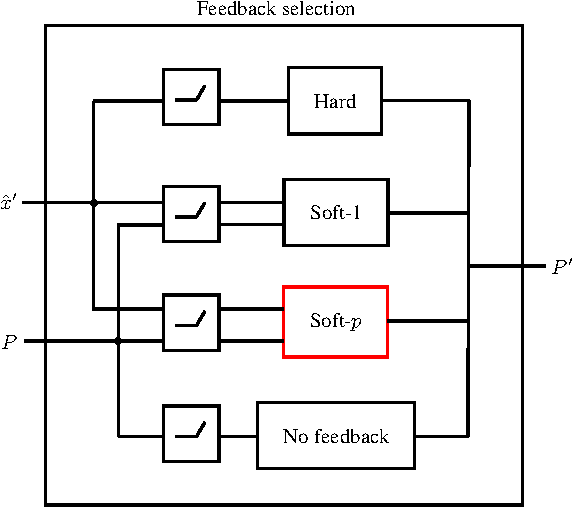
\includegraphics{./figures/parts/02/chapters/02/sections/03/feedback}
  \caption{\small Εσωτερικά στην τροποποιημένη έκδοση του MCL υπάρχουν τέσσερις
           διαφορετικοί και αμοιβαίως αποκλειόμενοι τρόποι ανατροφοδότησης. Με
           $\hat{\bm{x}}^{\prime}$ συμβολίζεται η έξοδος της διαδικασίας
           ευθυγράμμισης σαρώσεων, με $\bm{P}$ ο πληθυσμός σωματιδίων του
           φίλτρου, και με $\bm{P}^{\prime}$ ο πληθυσμός του φίλτρου μετά την
           εφαρμογή της ανατροφοδότησης. Το κόκκινο χρώμα χρησιμοποιείται για να
           προσδιορίσει τη συμβολή της προσέγγισής μας σε σχέση με την
           ανατροφοδότηση σε συστήματα φίλτρων σωματιδίων συνδυασμένα με
           ευθυγράμμιση σαρώσεων της τρέχουσας βιβλιογραφίας}
  \label{fig:feedback}
\end{figure}

\begin{algorithm}
  \caption{\texttt{feedback\_selection}}
  \label{alg:feedback_selection}
  \begin{spacing}{1.2}
  \begin{algorithmic}[1]
    \REQUIRE $\bm{P}_t \equiv \{(\hat{\bm{x}}_t^i, w_t^i)\}$, $q$, $\hat{\bm{x}}^\prime_t$, feedback\_manner
    \ENSURE $\bm{P}_{t+1}$
    \STATE \texttt{assert} feedback\_manner $\in \{$\texttt{hard}, \texttt{soft\_1}, \texttt{soft\_p}, \texttt{open}$\}$
    \IF {feedback\_manner = \texttt{hard}}
      \STATE $\bm{P}_{t+1} \leftarrow \overbrace{\{\hat{\bm{x}}^\prime_t\} \cup \{\hat{\bm{x}}^\prime_t\} \cup \dots \{\hat{\bm{x}}^\prime_t\}}^{N_{\max}}$
      \STATE Perturb $\bm{P}_{t+1}.\hat{\bm{x}}_t^i$ according to MCL initialisation parameters
    \ENDIF
    \IF {feedback\_manner = \texttt{soft\_1}}
      \IF {$|\bm{P}_t| = N_{\max}$}
        \STATE $\bm{P}_t \leftarrow$ \texttt{sort} $\bm{P}_t$ by weight, ascending
        \STATE Delete $\bm{P}_t[0]$
      \ENDIF
      \STATE $\bm{\bm{P}}_{t+1} \leftarrow \bm{P}_t \cup \hat{\bm{x}}^\prime_t$
    \ENDIF
    \IF {feedback\_manner = \texttt{soft\_p}}
      \STATE \texttt{assert} $q \in (0,1)$
      \STATE $\bm{S} \leftarrow \{\}$
      \IF {$|\bm{P}_t| \leq (1-q) N_{\max}$}
        \STATE $\bm{S} \leftarrow \underbrace{\{\hat{\bm{x}}^\prime_t\} \cup \{\hat{\bm{x}}^\prime_t\} \cup \dots \{\hat{\bm{x}}^\prime_t\}}_{\left\lfloor\dfrac{q}{1-q}|\bm{P}_t|\right\rfloor}$
      \ELSIF {$|\bm{P}_t| = N_{\max}$}
        \STATE $\bm{P}_t \leftarrow$ \texttt{sort} $\bm{P}_t$ by weight, ascending
        \STATE Delete $\bm{P}_t[0: \left\lfloor qN_{\max} \right\rfloor-1]$
        \STATE $\bm{S} \leftarrow \underbrace{\{\hat{\bm{x}}^\prime_t\} \cup \{\hat{\bm{x}}^\prime_t\} \cup \dots \{\hat{\bm{x}}^\prime_t\}}_{\left\lfloor qN_{\max}\right\rfloor}$
      \ELSE
        \STATE $\bm{P}_t \leftarrow$ \texttt{sort} $\bm{P}_t$ by weight, ascending
        \STATE Delete $\bm{P}_t[0: \left\lfloor |\bm{P}_t| - (1-q)N_{\max} \right\rfloor-1]$
        \STATE $\bm{S} \leftarrow \underbrace{\{\hat{\bm{x}}^\prime_t\} \cup \{\hat{\bm{x}}^\prime_t\} \cup \dots \{\hat{\bm{x}}^\prime_t\}}_{\left\lfloor qN_{\max}\right\rfloor}$
      \ENDIF
      \STATE $\bm{P}_{t+1} \leftarrow \bm{P}_{t} \cup \bm{S}$
    \ENDIF
    \IF {feedback\_manner = \texttt{open}}
      \STATE {$\bm{P}_{t+1} \leftarrow \bm{P}_t$}
    \ENDIF
    \RETURN $\bm{P}_{t+1}$
  \end{algorithmic}
  \end{spacing}
\end{algorithm}



%%%%%%%%%%%%%%%%%%%%%%%%%%%%%%%%%%%%%%%%%%%%%%%%%%%%%%%%%%%%%%%%%%%%%%%%%%%%%%%%
\subsection{Το ολικό σύστημα ελάττωσης του σφάλματος εκτίμησης}
\label{subsection:02_02_03:04}

Η δομή του ολικού συστήματος ελάττωσης του σφάλματος εκτίμησης της στάσης ενός
φίλτρου σωματιδίων απεικονίζεται στο σχήμα \ref{fig:overall_system}.  Το
προτεινόμενο συνολικό σύστημα είναι πιο ευέλικτο από έναν συνδυασμό φίλτρου
σωματιδίων με δειγματοληψία KLD και ευθυγράμμιση πραγματικών με εικονικές
σαρώσεις, καθώς αυτή είναι μία ειδική περίπτωση του προτεινόμενου συστήματος:
επιλέγοντας $100\%$ των σωματιδίων από τον πληθυσμού του MCL για την εξαγωγή
της εκτίμησης της στάσης του και δίχως ανατροφοδότηση, το προκύπτον σύστημα
μεταβάλλεται στην απλούστερη περίπτωση του εισαγόμενου συστήματος, δηλαδή στον
απλό MCL με δειγματοληψία KLD. Επιπρόσθετα, οι δύο προσεγγίσεις που
παρουσιάζονται στα \cite{Vasiljevic2016a} και \cite{Peng2018a} αποτελούν
ειδικές διαμορφώσεις του προτεινόμενου συστήματος. Στη συνέχεια, όταν
αναφερόμαστε στην εκτίμηση της στάσης που εξάγεται από τον MCL θα αναφερόμαστε
στην $\hat{\bm{x}}_t$, και όταν αναφερόμαστε στην έξοδο του συστήματος, ή του
σύνθετου συστήματος, ή του συνολικού συστήματος, θα αναφερόμαστε στην εκτίμηση
$\hat{\bm{x}}^{\prime}_t$.

\begin{figure}[h]\centering
  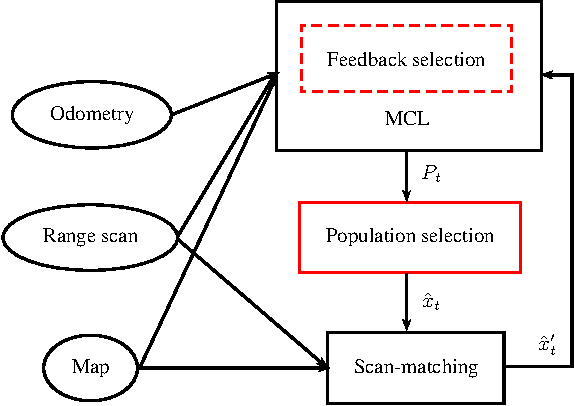
\includegraphics{./figures/parts/02/chapters/02/sections/03/overall_system}
  \caption{\small Το συνολικό σύστημα που στοχεύει στην επίλυση του προβλήματος
           \ref{prob:02_02:the_problem} υπό την Παραδοχή
           \ref{assumption:02_02_01:01} σε δομή μπλοκ. Τα παραλληλόγραμμα
           υποδεικνύουν υποσυστήματα, ενώ οι ελλείψεις τις εισόδους τους. Το
           κόκκινο χρώμα χρησιμοποιείται για να προσδιορίσει τα σημεία των
           συμβολών της προσέγγισής μας στα συστήματα συνδυασμού φίλτρων
           σωματιδίων με ευθυγράμμιση πραγματικών και εικονικών σαρώσεων
           αισθητήρα lidar δισδιάστατων μετρήσεων. Εδώ η ευθυγράμμιση σαρώσεων
           αντιμετωπίζεται ως προσθετικό σύστημα του MCL. Ο πληθυσμός του MCL
           $\bm{P}_t$ υπόκειται σε πιθανή διαλογή σωματιδίων τη χρονική στιγμή
           $t>0$. Η εκτίμηση εξόδου του μηχανισμού διαλογής προκύπτει από τον
           σταθμισμένο μέσο όρο των στάσεων των επιλεγμένων στάσεων. Η
           προκύπτουσα στάση χρησιμοποιείται ως η στάση από την οποία
           συλλαμβάνεται μία εικονική σάρωση εντός του χάρτη. Η πραγματική και
           η εικονική σάρωση ευθυγραμμίζονται στη συνέχεια χρησιμοποιώντας έναν
           αλγόριθμο ευθυγράμμισης πραγματικών με εικονικές (ή πραγματικές)
           σαρώσεις (εδώ τον αλγόριθμο ευθυγράμμισης πραγματικών σαρώσεων
           PLICP). Η έξοδος της διαδικασίας ευθυγράμμισης
           $\hat{\bm{x}}^{\prime}_t$ είναι, καταρχήν, πιο ακριβής από εκείνη
           του MCL, $\hat{\bm{x}}_t$, το οποίο σημαίνει ότι θα μπορούσε να
           χρησιμοποιηθεί ως βοηθητικό μέσο ελάττωσης του σφάλματος εκτίμησης
           του ίδιου το MCL με την ανατροφοδότησή της πίσω στον πληθυσμό του}
  \label{fig:overall_system}
\end{figure}
